\section{General design}

\subsection{Use case diagram}

\begin{figure}[H]
  \centering
  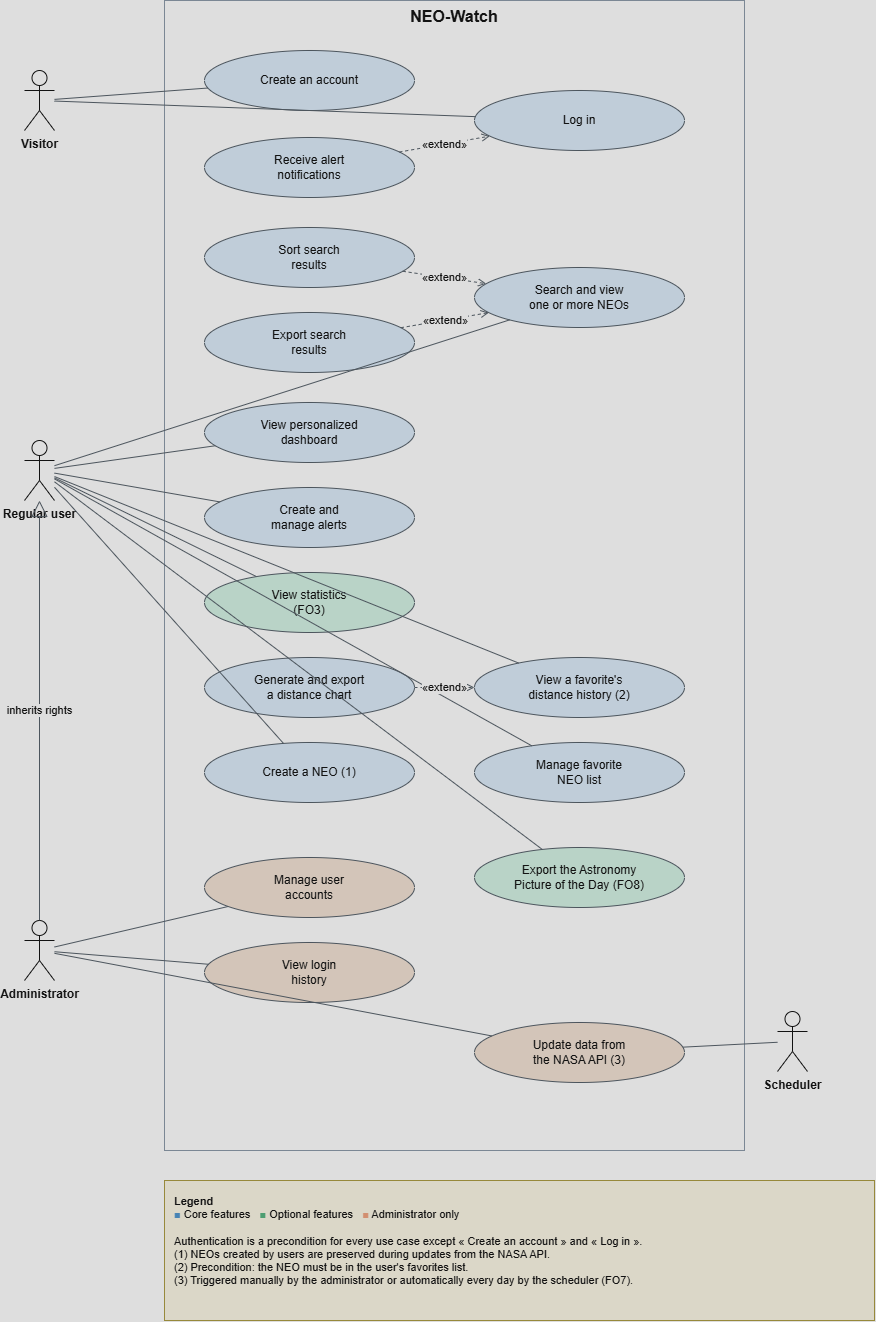
\includegraphics[width=0.8\textwidth]{figures/use_case_diagram_en_final.png}
  \caption{Use case diagram}
  \label{fig:use-case-diagram}
\end{figure}

\label{sec:use-case-diagram}


The diagram shown in figure~\ref{fig:use-case-diagram} distinguishes three
actors.

The visitor only has access to account creation and login,
since the application is secured.
The regular user has access to
the full set of consultation and personalization features:
dashboard, search and export, creation of an observed NEO, management of
their favorites and the associated distance charts, definition of alerts and
receipt of the corresponding notifications upon login.
The administrator inherits these rights and adds account management, viewing
the login history, and triggering the data update.

This inheritance relationship reflects the fact that an administrator is
first and foremost a user, which avoids duplicating some fifteen use cases
and is reflected in the model as a simple role attribute rather than a
class hierarchy.

\subsection{Layered architecture}

The layered architecture is the foundation of our application. Each task required by the application is distributed between the different layers which have different roles.

The first one is the frontend. Its role is the only layer that users see and interact with. It shows everything that has to be displayed. In addition, it is also where people can press the buttons in order to navigate in the app. He will be able to choose the features he wants to try. Once the function is chosen, the request goes to the controller which is part of the backend.

The controller receives and sends https requests from the frontend, like the choice of users, or from the API. Its role is to link the API with the service, which is where all the process truly happens. In the classes Service, we have all the methods in order to make our application useful. It is like the brain of the project. For example, that is where the statistics are calculated, we can also create or delete a NEO. But, to be able to do that, it needs the data. Therefore, at this moment, the service calls the DAO (Data Access Object). The DAO receives the request in python of the service, converts it in sql, and sends that to the database. Once the response from the table is arrived, it is translated back to python, in an object that the app understands, and given to the concerned service.


\subsection{Class diagram}

\label{sec:mpd}

\begin{figure}[H]
  \centering
  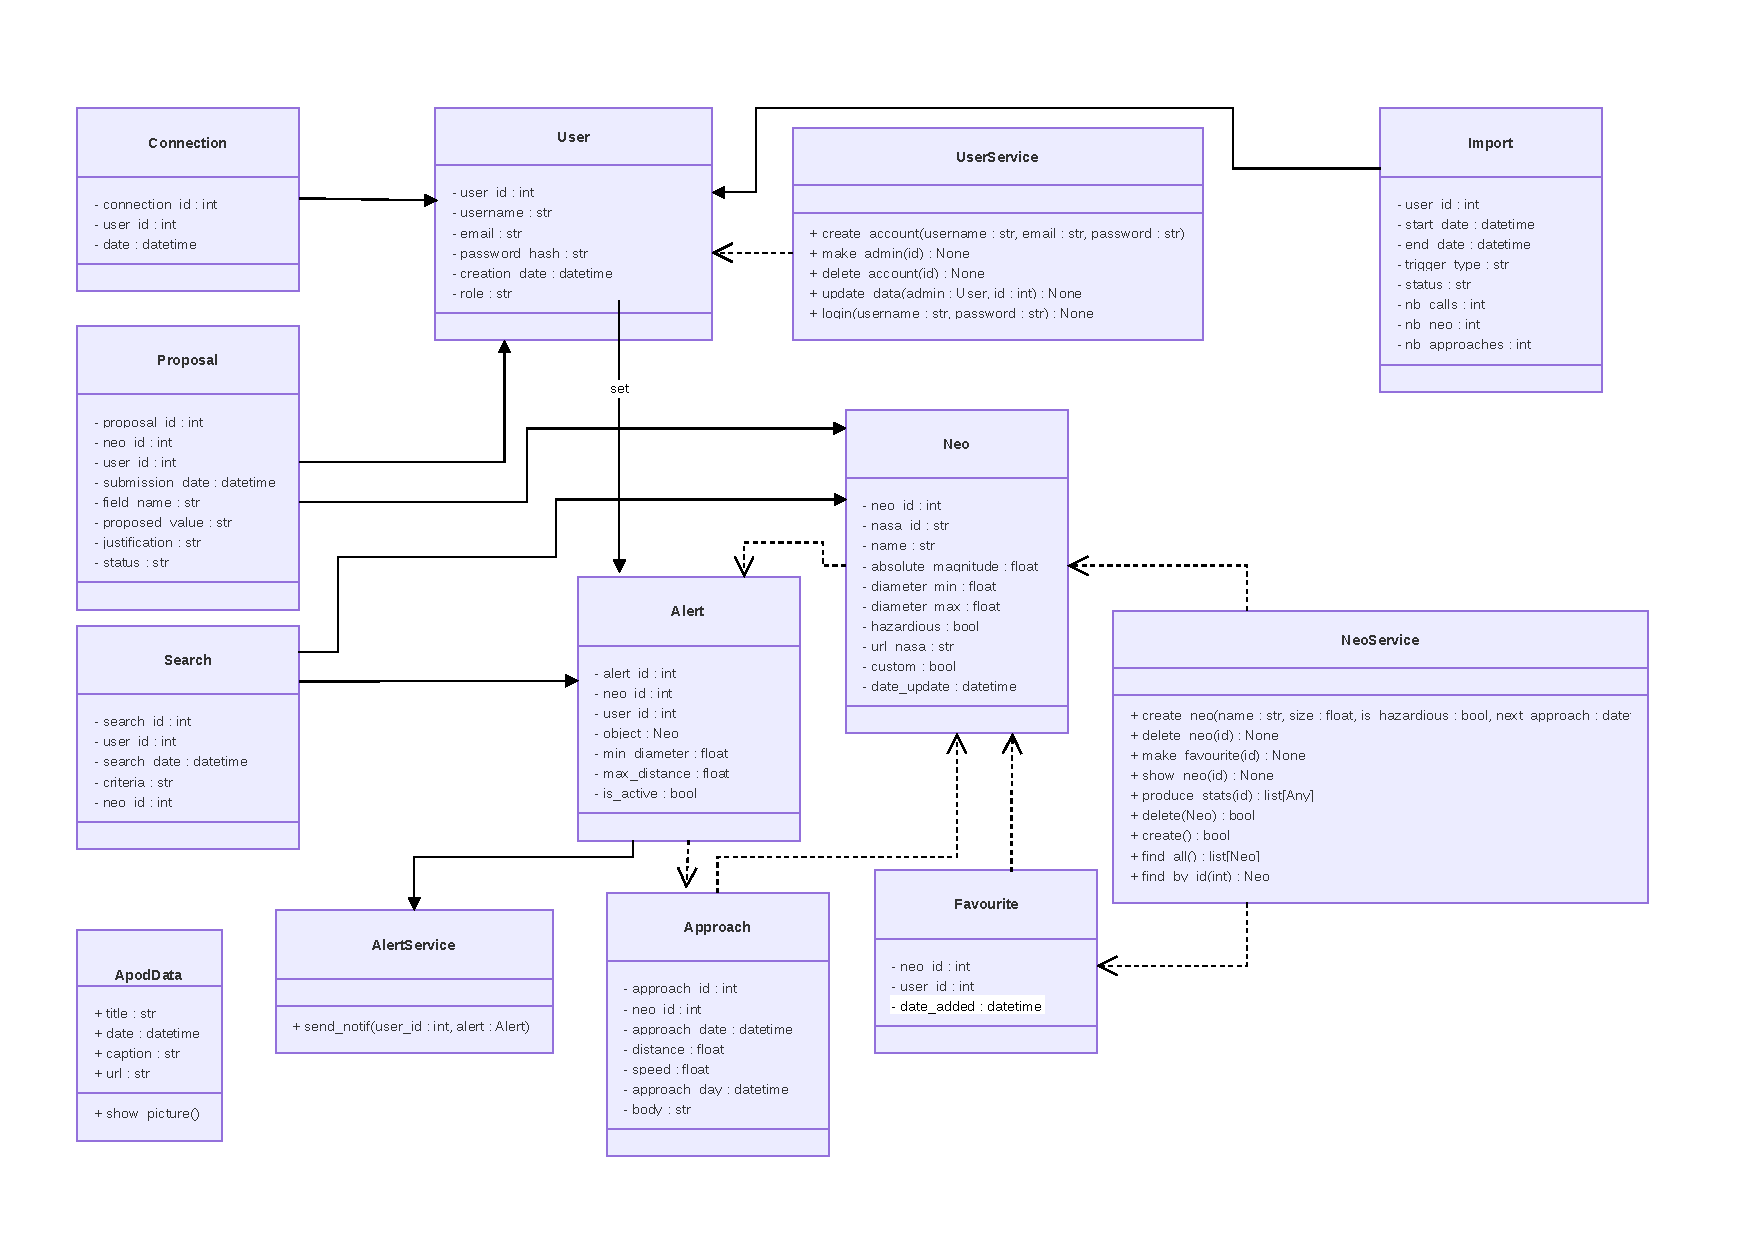
\includegraphics[width=0.8\textwidth]{figures/diag_class_pdf.drawio-7.pdf}
  \caption{Class diagram}
  \label{fig:class-diagram}
\end{figure}

\label{sec:class-diagram}

The class diagram contains most of the classes that we will need for the app. Many classes will be coded later, but we chose to show only these ones, because other classes about DAO or the controller for example, do not provide a lot of information as they are always present in this kind of app. What we can see is the heart of the project, it is the structure of all the functions provided by the app.

Moreover, except for the classes Neo and User; the classes that have been created will be used only in one function. Even if we wanted to gather them as much as possible, in order to simplify our app, as all the functions are pretty different, we could not reduce their count.

Among all these, one class is isolated from the others. ApodData is the class that will fulfill the features of displaying the Picture of the Day. As its only role is to show this picture to the user, there is no link between an user information or a Neo, the class does not need any link.



\subsection{Physical data model}
\label{sec:mpd}

\begin{figure}[H]
  \centering
  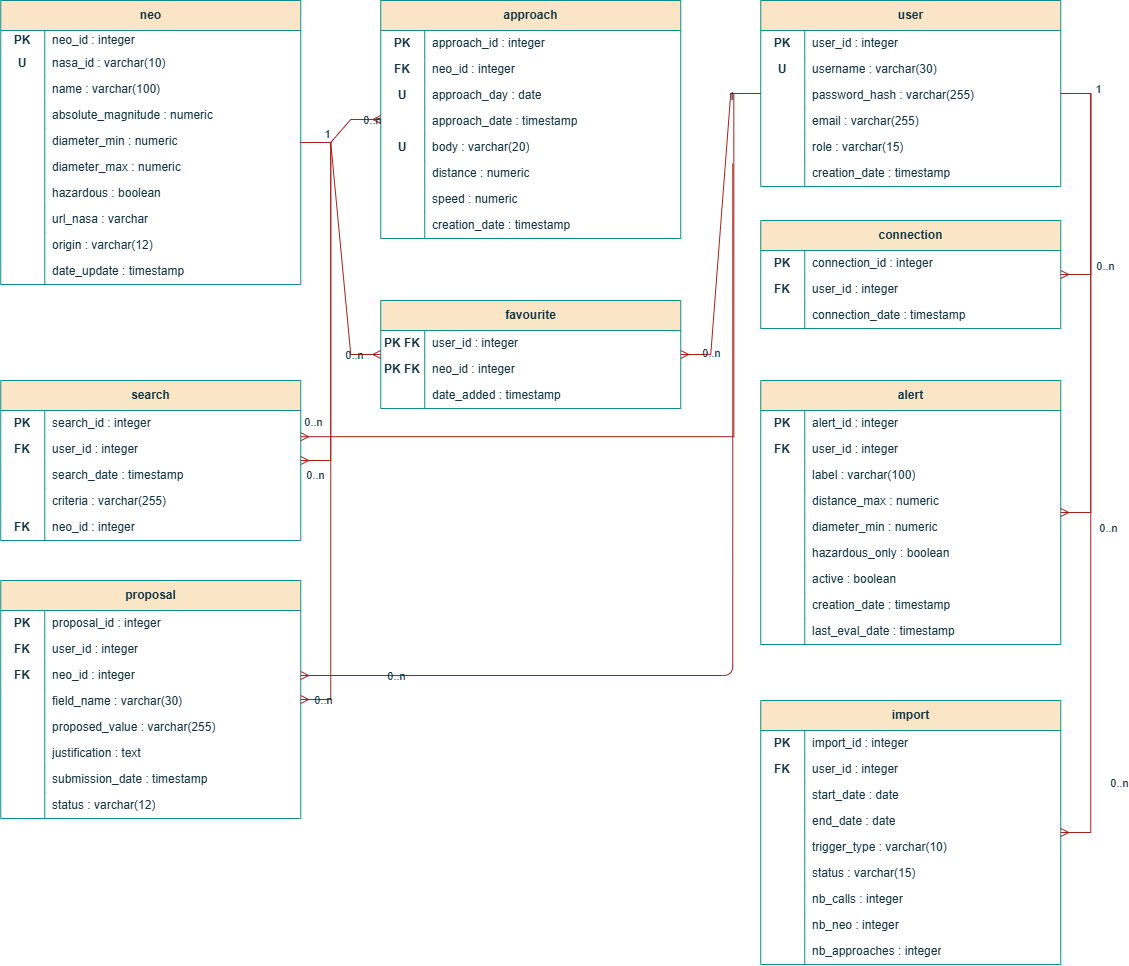
\includegraphics[width=0.8\textwidth]{figures/databasediag.png}
  \caption{Physical data model}
  \label{fig:data-base-diagram}
\end{figure}

\label{sec:data-base-diagram}


The model is built on nine tables, organized around two central entities.
The \texttt{neo} table holds the stable characteristics of a near-Earth
object, and the \texttt{approach} table its successive close passes near
a body of the solar system. A NEO has zero to several close approaches,
and each close approach concerns exactly one NEO.

\paragraph{Two tables rather than one.}
For each NEO, the API returns a list of dated close approaches, along with
their distance and speed : the same object appears several times
over a given period. A single table would have duplicated the physical
characteristics at each of these approaches. Beyond the volume, the main
risk concerns updates : diameter, magnitude and the hazard flag are
regularly revised by NASA, and it would have been necessary to modify the
twenty-nine rows of an object without error. We therefore split the data into
two tables, \texttt{neo} and \texttt{approach}, linked by a foreign key.
The decisive argument, however, is referential integrity: a favorite, an
alert, or a proposed correction relates to a NEO and not to a close
approach, and without a \texttt{neo} table these relationships would have
no stable target to reference.

\paragraph{Primary keys and uniqueness constraints.}
The identifier provided by NASA guarantees uniqueness, but feature F4
allows a user to create a NEO they have observed themselves, and by
definition such an object has no NASA identifier. We therefore use an
auto-incremented technical key, and keep the NASA identifier in a
separate column, nullable and subject to a uniqueness constraint.
Imported objects and user-created objects thus coexist in the same table
without either case having to be treated as an exception.

\paragraph{Identifying close approaches.}
The API provides no approach identifier. A close approach is therefore
recognized by the triplet formed by the object, the day of the pass, and
the body approached, on which a uniqueness constraint is placed. The day
is used rather than the full timestamp because successive refinements of
the orbital solutions shift the announced time : a key
based on the timestamp would produce a duplicate at each update, whereas
two passes of the same object toward the same body on the same day are
physically impossible. The precise timestamp is still kept, for display
purposes. All dates are expressed in Coordinated Universal Time as used
by the API.

\paragraph{Preserving user-created objects.}
A refresh would overwrite user-entered objects on every import. To
prevent this, we add an \texttt{origin} column to the \texttt{neo}
table, which takes the value \texttt{NASA} or \texttt{USER}. The
insert or update query executed during an import is restricted by a
\texttt{WHERE origin = 'NASA'} clause, which makes user-created entries
not affected by successive reloads.

\paragraph{The relationship between users and objects.}
The \texttt{favourite} table resolves the many-to-many relationship between
users and objects, a user being able to follow several NEOs and a NEO
being followed by several users. Its composite primary key inherently
prevents the same object from being favorited twice by the same person.
The date of addition belongs to the link itself rather than to either entity,
and is therefore stored in the association table.

\paragraph{Storing statistics.}
The statistics expected in FO3 :  number of hazardous objects over a
period, minimum distance, averages, could be precomputed in a table
refreshed at each import, which would speed up display. We chose the
opposite solution: only raw data is stored, and all aggregates are
computed in SQL at query time. The import window represents a few tens
of thousands of approach rows, a volume for which aggregation on
PostgreSQL is immediate, and this solution avoids maintaining a
redundancy that would need to be invalidated at every update. The cost is
a longer response time as the window widens, which we consider
acceptable at the scale of this project.

\paragraph{Import traceability.}
Finally, the \texttt{import} table keeps a record of each data load. It
allows the administrator to view its history, as required by F1, and
allows the application to know the period actually covered by the
database before answering a request for statistics over a period that
may not have been imported.

\subsubsection{Variable dictionary}

\begin{longtable}{@{}p{0.24\linewidth}p{0.17\linewidth}p{0.51\linewidth}@{}}
\toprule
\textbf{Variable} & \textbf{Type} & \textbf{Description} \\
\midrule
\endfirsthead
\toprule
\textbf{Variable} & \textbf{Type} & \textbf{Description} \\
\midrule
\endhead
\bottomrule
\endfoot

\multicolumn{3}{@{}l}{\textbf{neo} --- stable characteristics of a near-Earth object} \\
\midrule
\texttt{neo\_id} & integer & Technical primary key \\
\texttt{nasa\_id} & varchar(10) & NASA identifier, empty if the object was created by a user \\
\texttt{name} & varchar(100) & Name or provisional designation of the object \\
\texttt{absolute\_magnitude} & numeric & Intrinsic brightness of the object \\
\texttt{diameter\_min} & numeric & Lower bound of the estimated diameter, in meters \\
\texttt{diameter\_max} & numeric & Upper bound of the estimated diameter, in meters \\
\texttt{hazardous} & boolean & Object classified as potentially hazardous by NASA \\
\texttt{url\_nasa} & varchar & Link to the official JPL page \\
\texttt{origin} & varchar(12) & \texttt{NASA} or \texttt{USER} \\
\texttt{date\_update} & timestamp & Date of the row's last refresh \\
\addlinespace
\midrule

\multicolumn{3}{@{}l}{\textbf{approach} --- close pass of an object near a body} \\
\midrule
\texttt{approach\_id} & integer & Technical primary key \\
\texttt{neo\_id} & integer & Object concerned \\
\texttt{approach\_day} & date & Day of the pass, in UTC \\
\texttt{approach\_date} & timestamp & Precise timestamp of the pass \\
\texttt{body} & varchar(20) & Body approached, Earth within our scope \\
\texttt{distance} & numeric & Minimum distance reached, in kilometers \\
\texttt{speed} & numeric & Relative speed at the time of the pass \\
\texttt{creation\_date} & timestamp & Date the row was inserted into the database \\
\addlinespace
\midrule

\multicolumn{3}{@{}l}{\textbf{user} --- account for accessing the application} \\
\midrule
\texttt{user\_id} & integer & Technical primary key \\
\texttt{username} & varchar(30) & Login identifier, unique \\
\texttt{password\_hash} & varchar(255) & Password hash \\
\texttt{email} & varchar(255) & Contact address \\
\texttt{role} & varchar(15) & \texttt{USER} or \texttt{ADMIN} \\
\texttt{creation\_date} & timestamp & Registration date \\
\addlinespace
\midrule

\multicolumn{3}{@{}l}{\textbf{favourite} --- association between a user and a followed object} \\
\midrule
\texttt{user\_id} & integer & User concerned \\
\texttt{neo\_id} & integer & Object marked as favorite \\
\texttt{date\_added} & timestamp & Date the favorite was added \\
\addlinespace
\midrule

\multicolumn{3}{@{}l}{\textbf{connection} --- login history} \\
\midrule
\texttt{connection\_id} & integer & Technical primary key \\
\texttt{user\_id} & integer & Account concerned \\
\texttt{connection\_date} & timestamp & Date and time of login \\
\addlinespace
\midrule

\multicolumn{3}{@{}l}{\textbf{alert} --- monitoring criteria defined by a user} \\
\midrule
\texttt{alert\_id} & integer & Technical primary key \\
\texttt{user\_id} & integer & Owner of the alert \\
\texttt{label} & varchar(100) & Name given by the user \\
\texttt{distance\_max} & numeric & Proximity threshold, empty if this criterion is not used \\
\texttt{diameter\_min} & numeric & Size threshold, empty if this criterion is not used \\
\texttt{hazardous\_only} & boolean & Restricts the alert to objects classified as hazardous \\
\texttt{active} & boolean & Allows the alert to be suspended without deleting it \\
\texttt{creation\_date} & timestamp & Date the alert was defined \\
\texttt{last\_eval\_date} & timestamp & Last evaluation, avoids reporting the same event twice \\
\addlinespace
\midrule

\multicolumn{3}{@{}l}{\textbf{import} --- record of loads from the NASA API} \\
\midrule
\texttt{import\_id} & integer & Technical primary key \\
\texttt{user\_id} & integer & Triggering administrator, empty if the import is automatic \\
\texttt{start\_date} & date & Start of the imported period \\
\texttt{end\_date} & date & End of the imported period \\
\texttt{trigger\_type} & varchar(10) & \texttt{MANUAL} or \texttt{BATCH} \\
\texttt{status} & varchar(15) & \texttt{N
ON\_GOING}, \texttt{DONE}, \texttt{PARTIAL}, or \texttt{FAIL} \\
\texttt{nb\_calls} & integer & Number of calls made to the API \\
\texttt{nb\_neo} & integer & Number of objects inserted or updated \\
\texttt{nb\_approaches} & integer & Number of close approaches inserted or updated \\
\addlinespace
\midrule

\multicolumn{3}{@{}l}{\textbf{search} --- search history, kept for thirty days} \\
\midrule
\texttt{search\_id} & integer & Technical primary key \\
\texttt{user\_id} & integer & Author of the search \\
\texttt{search\_date} & timestamp & Timestamp of the search \\
\texttt{criteria} & varchar(255) & Criteria entered, in readable text \\
\texttt{neo\_id} & integer & Object viewed, empty if this is a multi-criteria search \\
\addlinespace
\midrule

\multicolumn{3}{@{}l}{\textbf{proposal} --- correction suggested by a user} \\
\midrule
\texttt{proposal\_id} & integer & Technical primary key \\
\texttt{user\_id} & integer & Author of the proposal \\
\texttt{neo\_id} & integer & Object concerned \\
\texttt{field\_name} & varchar(30) & Field the user wants corrected \\
\texttt{proposed\_value} & varchar(255) & Suggested value \\
\texttt{justification} & text & Free-text explanation \\
\texttt{submission\_date} & timestamp & Date the proposal was submitted \\
\texttt{status} & varchar(12) & \texttt{WAITING}, \texttt{READ}, or \texttt{REJECTED} \\
\end{longtable}


\subsection{Packages diagram}

The application is built upon a strict layered architecture to separate concerns and ensure maintainability. The \texttt{FRONTEND}, built with Streamlit, manages the user interface and captures user inputs. It communicates via HTTP requests with the \texttt{CONTROLLER} layer, handled by FastAPI. The controller routes these requests to the \texttt{SERVICE LAYER}, which acts as the "brain" of the project, executing the core business logic and interacting with the external NASA API when data updates are required. Finally, the \texttt{DAO} (Data Access Object) is responsible for data persistence. It translates Python commands into SQL queries to interact with the local PostgreSQL \texttt{DATABASE}.


\begin{figure}[H]
  \centering
  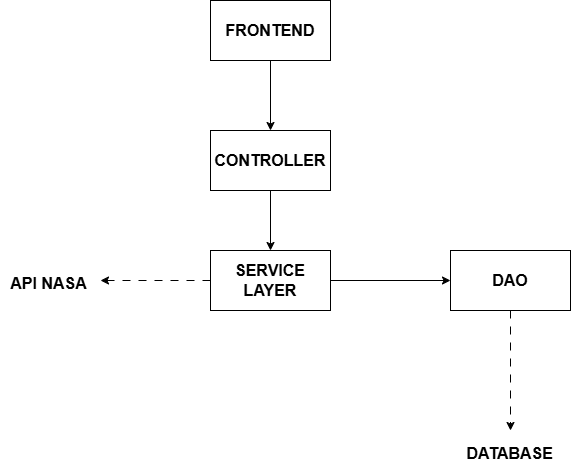
\includegraphics[width=0.8\textwidth]{figures/diagramme_packages.drawio.png}
  \caption{Packages diagram}
  \label{fig:packages-diagram}
\end{figure}

\subsection{Sequence diagram}

This sequence diagram details the internal execution flow when a user searches for near-Earth objects based on specific criteria. When the search is submitted, the request travels from the Streamlit frontend down to the service layer. The DAO then executes a SQL JOIN query between the neo and approach tables in the local PostgreSQL database. This read operation relies entirely on our pre-populated database and does not trigger any external calls to the NASA API.  The diagram highlights two alternative outcomes using an alt block: if matches are found, the data is formatted and passed back to the frontend to be displayed as a sortable table. An opt (optional) block illustrates the CSV export feature, which is handled purely on the client side without querying the database again. If no NEO matches the criteria, the system propagates an empty list back to the user interface to display a "No results found" message. 



\begin{sidewaysfigure}
    \centering
    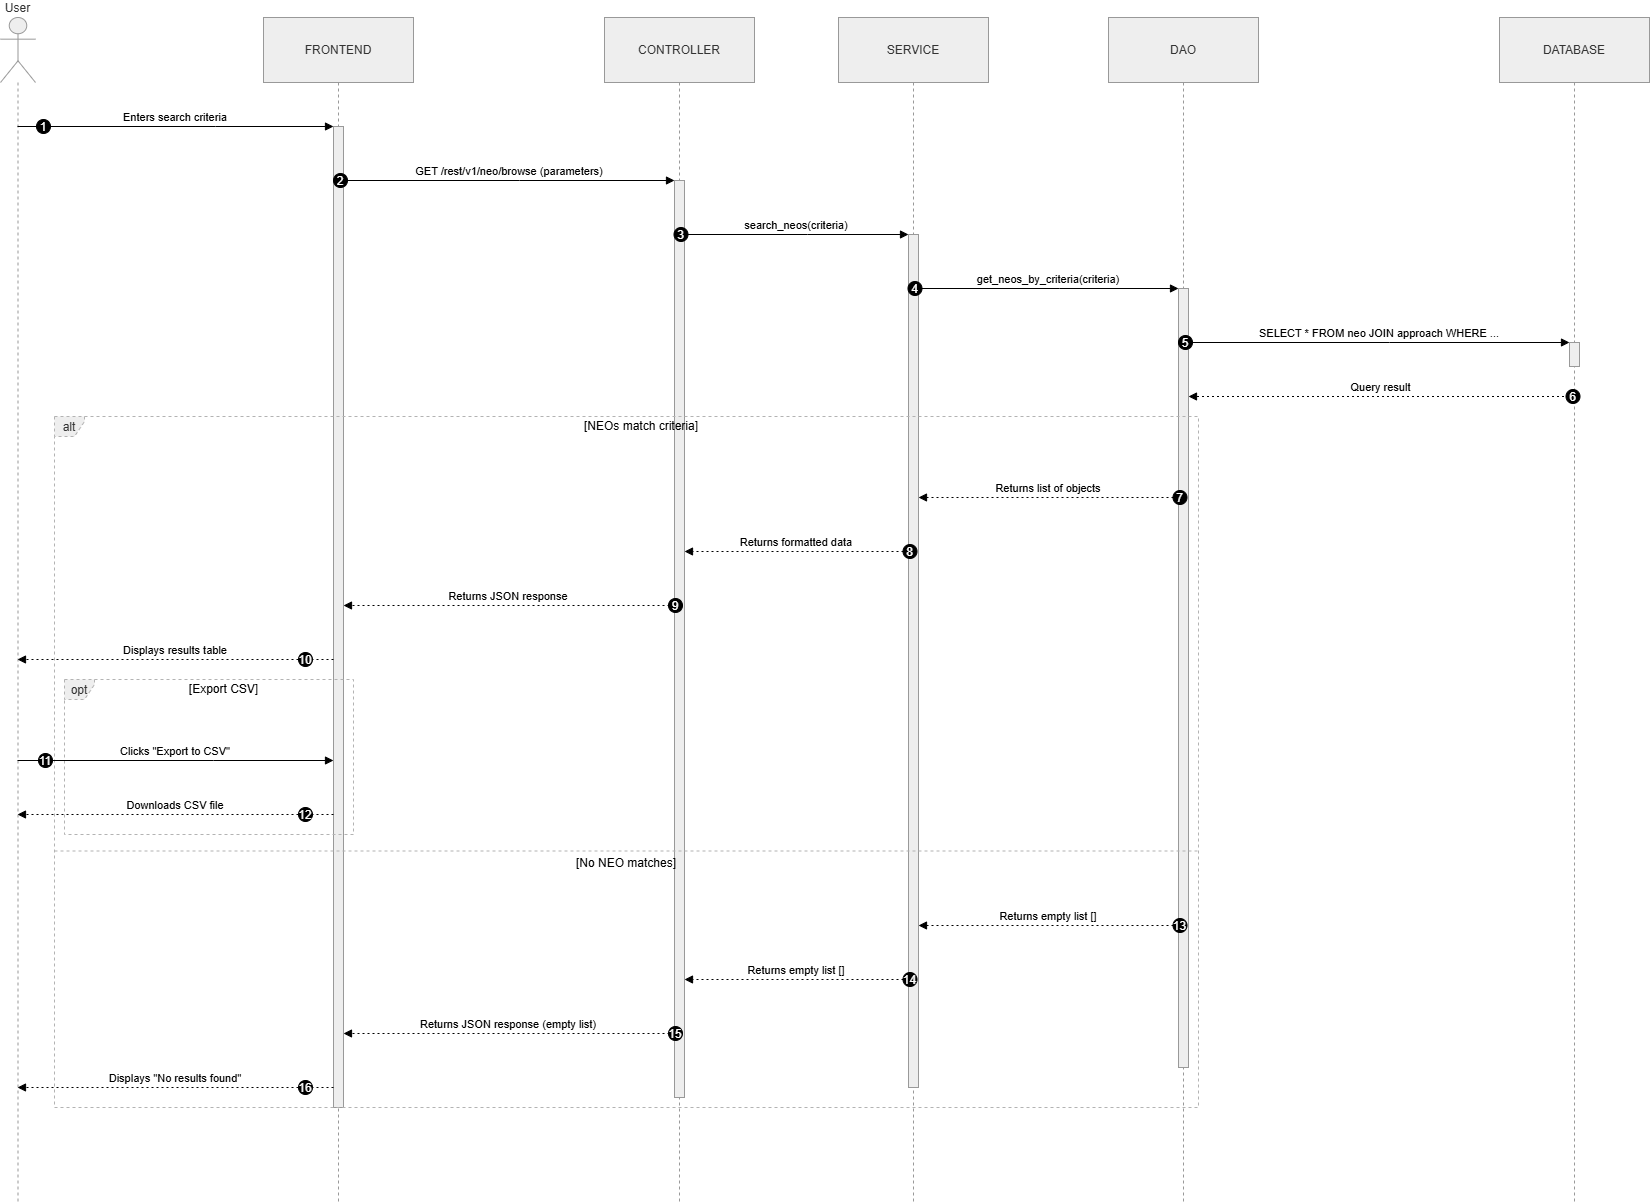
\includegraphics[width=\textwidth]{figures/diagramme_sequence.drawio.png}
    \caption{Sequence diagram for NEO Search (F3)}
    \label{fig:seq_search}
\end{sidewaysfigure}

\subsection{Streamlit screens}

NEO-Watch's frontend will be built with Streamlit. As no screens have been implemented yet, this section presents the planned screen structure, derived from the choices made in section 2.2.

\paragraph{Home / Dashboard.}
Entry point after login. Lists upcoming approaches within a selectable window, the count of potentially dangerous NEOs among them (flagged via the API's \texttt{is\_potentially\_hazardous\_asteroid} field), and the closest NEO to Earth over a set period (F2), alongside the user's favorites and shortcuts to search, favorites and alerts.

\paragraph{Search.}
Lets the user query approaches over a date range, by name, id, dimensions or date (F3). Results are shown as a sortable table (distance in km and AU, speed in km/h) with a CSV export button, built directly from stored data with no additional call to the NASA API.

\paragraph{NEO detail page.}
Full record for one object: diameter range as returned by the API, distances, an "add to favorites" action, and for favorites, the distance history retrieved via \texttt{/neo/id} (F5), with CSV export of the history graph.

\paragraph{Create a NEO.}
Form for user-submitted observations (F4), limited to the fields an amateur observer can realistically provide; submitted objects are tagged \texttt{origin = USER} to protect them from the daily NASA import.

\paragraph{Alerts.}
Lets the user define and manage notification criteria (diameter, distance thresholds) (F6), and view past notifications received at login.

\paragraph{Statistics (FO3).}
Distributions over the objects currently in the database (size, share of hazardous objects), computed on demand in SQL rather than pre-aggregated.

\paragraph{Picture of the Day (FO8).}
Displays the NASA APOD image and description.

\paragraph{Admin panel.}
Account management and connection history (F1), a manual "trigger update" button calling the same service as the scheduled daily job (FO7), and the status of the current/last import.


\subsection{Endpoint table}

The following table details the endpoints:

\begin{table}[htbp]
    \centering
    \begin{tabular}{|l|p{9cm}|}
        \hline
        \textbf{Endpoint} & \textbf{Description} \\
        \hline
        \texttt{POST /api/v1/auth/login} & Authenticate a user (regular or administrator) and initiate a session. \\
        \hline
        \texttt{GET /api/v1/dashboard} & Retrieve personalized dashboard metrics (upcoming approaches, hazardous NEOs count, closest NEO). \\
        \hline
        \texttt{GET /api/v1/neos} & Search the local database for NEOs and approaches based on query parameters (name, dates, dimensions). \\
        \hline
        \texttt{GET /api/v1/neos/\{neo\_id\}} & Retrieve detailed characteristics and the complete close approach history for a specific NEO. \\
        \hline
        \texttt{POST /api/v1/neos} & Submit a new amateur observation to create a custom NEO in the database. \\
        \hline
        \texttt{GET /api/v1/users/me/favorites} & Get the authenticated user's list of favorite NEOs. \\
        \hline
        \texttt{POST /api/v1/users/me/favorites/\{neo\_id\}} & Add a specific NEO to the user's favorites list. \\
        \hline
        \texttt{DELETE /api/v1/users/me/favorites/\{neo\_id\}} & Remove a NEO from the user's favorites list. \\
        \hline
        \texttt{GET /api/v1/users/me/alerts} & Retrieve the user's active alert configurations and any pending notifications. \\
        \hline
        \texttt{POST /api/v1/users/me/alerts} & Create a new alert configuration (e.g., minimum diameter, maximum distance). \\
        \hline
        \texttt{GET /api/v1/stats} & Compute and retrieve global statistics (size distribution, hazardous proportion) from the local database. \\
        \hline
        \texttt{POST /api/v1/admin/import} & Trigger a manual data update pulling the latest data from the NASA API into the local database. \\
        \hline
    \end{tabular}
    \caption{Endpoints requiring user identification utilize the \texttt{/users/me/} path, ensuring secure and isolated access to personal favorites and alerts. The \texttt{/api/v1/admin/import} route is restricted to administrator accounts. }
    \label{tab:endpoints}
\end{table}


